% !TeX root = ../praktikum.tex
% !TeX encoding = UTF-8
% !Tex spellcheck = de_DE



\subsection{Untersuchungen an Gittern}
In diesem Abschnitt werden verschiedene Gitter des Objektes 3 untersucht. Dazu wurde das entsprechende Dia in der Objektebene montiert. Das gewünschte Motiv auf der Schablone wurde möglichst mittig in dem Strahl montiert. Mit einer Papierschablone wurde verhindert, das Motive beleuchtet werden, die gerade nicht untersucht wurden, da dies eine Überlagerung mehrerer Fourierspektren zur Folge hätte (vgl. Abb.~\ref{fig:kreuzgitter_und_spektrum}~a und b) und das Untersuchen eines einzelnen Spektrums unmöglich machen würde. Für jedes der neun Motive wurde je ein Bild in der Fourierebene sowie in der Abbildungsebene aufgenommen. Bei dem Einschieben der Objekte lässt sich feststellen, dass die Bewegungsrichtung der Abbildung entgegengesetzt zu der des echten Motives ist. Ebenso sieht man bei asymmetrischen Objekten, dass diese "auf dem Kopf stehen".


\begin{figure}[ht]
	\centering
	%\includegraphicsRS[width=0.6\textwidth]{images/Regina/abb13.jpg}
	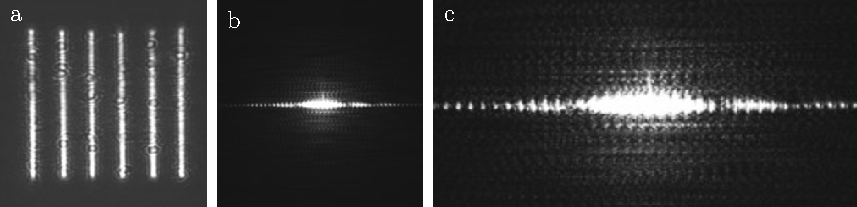
\includegraphics{images/Regina/abb13.pdf}
	\caption[Gitter mit Fourierspektrum]{
		Vertikales Gitter (a) und das dazugehörige Beugungsbild (b), welches das Fourierspektrum darstellt. Das Fourierspektrum weist erneut Beugungsbilder als eine Unterstruktur auf (c).
	}
	\label{fig:gitter_und_spektrum}
\end{figure}

Für eines der Gittermotive aus der ersten Reihe sind diese Aufnahmen in Abbildung~\ref{fig:gitter_und_spektrum} abgebildet. In der Fourierebene ist eine Reihe von Punkten zu sehen. Die Motive der zweiten Reihe ergeben in beiden Ebenen jeweils das gleiche Bild, jedoch um $90^\circ$ gedreht. Je dichter die Gitterlinien beieinander liegen, desto weiter liegen die Punkte in der Fourierebene auseinander.

Die Abbildung eines Motiv der letzten Reihe (Kreuzgitter) ist in Abbildung~\ref{fig:kreuzgitter_und_spektrum}~a abgebildet, b zeigt das Bild in der Fourierebene (\textit{Fourierspektrum}). Zusätzlich zeigt die Abbildung~\ref{fig:kreuzgitter_und_spektrum}c das Fourierspektrum, wenn mehrere Motive gleichzeitig beleuchtet werden. Die Kreuzgitter erzeugen in der Fourierebene zwei senkrechte Punktreihen, wobei der Punktabstand mit zunehmenden Gitterlinienabstand abnimmt.

\begin{figure}[ht]
	\centering
	%\includegraphicsRS[width=0.4\textwidth]{images/Regina/abb14.jpg}
	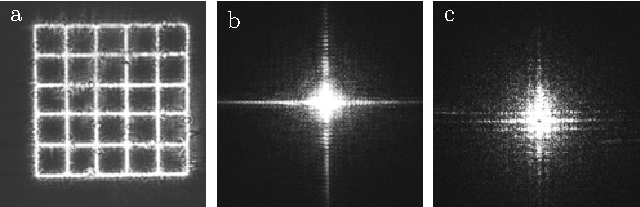
\includegraphics{images/Regina/abb14.pdf}
	\caption[Kreuzgitter mit Fourierspektrum]{
		Kreuzgitter (a) und das dazugehörige Beugungsbild (b), das das Fourierspektrum darstellt. Eine Überlagerung von mehreren Fourierspektren (c).
	}
	\label{fig:kreuzgitter_und_spektrum}
\end{figure}



\subsubsection*{Auswertung}
Das Zustandekommen und Aussehen einer Abbildung kann durch die aus der zweifachen 
Da das Licht im vertikalen Gitter nur in der vertikalen Richtung gebeugt wird, bilden sich die Intensitätsschwankungen in der Fourierebene ausschließlich in horizontaler Richtung aus. Somit wurde dort eine senkrecht zu dem Gitter stehende Reihe aus Interferenzmaxi- und -minima beobachtet: Vergleich Abbildung~\ref{fig:gitter_und_spektrum}. Das Drehen des Motives sorgt ebenfalls für ein gedrehtes Bild in der Fourierebene. Dies ist direkt aus der Beugungstheorie an Gittern ersichtlich. Die Änderungen des Spektrums unter Variation des Spaltabstandes zu beobachten waren, lassen sich mit der mathematischen Eigenschaft der Ähnlichkeit der FT erklären (s. Abschnitt~\ref{chap:math_basic}), allerdings folgt auch dies direkt aus der Beugungstheorie an Gittern beziehungsweise Mehrfachspalten.\\

Bei einem Kreuzgitter findet die Beugung in horizontaler und vertikaler Richtung statt, welches einer Kreuzform in der Fourierebene entspricht. Das Motiv entspricht also einer Überlagerung zweier um $90^\circ$ gedrehten Gitter. Nach der mathematischen Eigenschaft der Linearität der FT (s. Abschnitt~\ref{chap:math_basic}) folgt somit auch die Überlagerung der entsprechenden Spektren. Dies war sehr gut zu beobachten.

Wenn mehrere Motive beleuchtet wurden ergab sich in der Fourierebene die in Abbildung~\ref{fig:kreuzgitter_und_spektrum}~c dargestellt kreuzförmige Anordnung. Diese zeigt nicht ein einzelnes Kreuz, sondern mehrere Kreuze mit einem bestimmten Abstand voneinander. Das Auftreten mehrerer Kreuze lässt sich analog mit der Linearitätseigenschaft der FT erklären.

Sowohl bei dem vertikalen Gitter als auch bei dem Kreuzgitter ist in der Fourierebene im Zentrum der Beugungsbilder eine maximale Intensität zu erkennen. Dieses Maximum entsteht durch das Kreuzen der mittleren horizontalen oder im Kreuzgitter der vertikalen und
horizontalen Beugungsbilder. Dabei ist bei jedem weiteren Kreuzpunkt erneut eine erhöhte Intensität zu erkennen, die aber nach außen hin abnimmt. Diese lässt sich ebenfalls bei einem
Doppelspalt beobachten, wobei das Intensitätsmaximum nullter Ordnung am stärksten ist und die Maxima höherer Ordnungen immer schwächer werden ($\nicefrac{sin(x)}{x}$). Dabei nimmt die Intensität im Zentrum mit zunehmen kleiner werdenden Gitterkonstante zu.
Weiterhin wiesen alle Intensitätsmaxima eine Unterstruktur auf. Diese Unterstrukturen entstehen durch die Interferenz der Haupt- und Nebenmaxima aller Spalte des Gitters. Somit entsteht im Gegensatz zu einem Doppelspalt das Beugungsbild eines Gitter aus Vielfachinterferenzen. Diese Eigenschaft entspricht der mathematischen geforderten Linearität. Denn das Beugungsbild eines Gitters kann somit durch das aufsummieren der einzelnen Beugungsbilder des Einzelspaltes erzeugt werden (siehe 1.1. Linearität%TODO:REF!!!
).


\subsection{Erzeugung von Beugungsbilder von Punkten}
\subsubsection*{Auswertung}

Bei der optische Fouriertransformation gilt für Punkte wie bereits für Gittern erläutert die Linearität, so dass das erzeugte Beugungsbild in der Fourierebene sich aus der Summe der Beugungsbilder der einzelnen Punkte ergibt. Das Beugungsbild eines Punktes besteht aus konzentrischen Ringen, dessen Breite und Intensität nach außen abnehmen. Durch das Verschiebungtheorem der Fouriertransformation ist gegeben, dass sich das Beugungsbild der beiden Punkte an einer Position befinden, trotz der unterschiedlichen Position der Punkte. Bei zwei Punkten ergibt sich somit erneut eine Vielfachinterferenz analog zum Gitter, welches erneut durch Unterstrukturen in den konzentrischen Ringen erkennbar wird (Abb.~\ref{fig:punktpaare_verschieden_und_spektren}~b, d). Mit zunehmenden Abstand zwischen den Punkten werden die Unterstrukturen feiner. Dieses entspricht dem Ähnlichkeitstheorem (siehe 1.1. Ähnlichkeit%TODO:REF!!!
), so dass mit zunehmenden Abständen der Punkte sich die Beugungsmaxima annähern, bzw. die Abstände zwischen diesen kleiner werden. Für ein Gitter bedeutet dieses, je größer die Gitterkonstante ist, d.h. je größer der Abstand zwischen den Spalten ist, desto kleiner wird der Abstand zwischen den einzelnen Maxima und Minima.

\begin{figure}[h]
	\centering
	%\includegraphicsRS[width=0.3\textwidth]{images/Regina/abb15.jpg}
	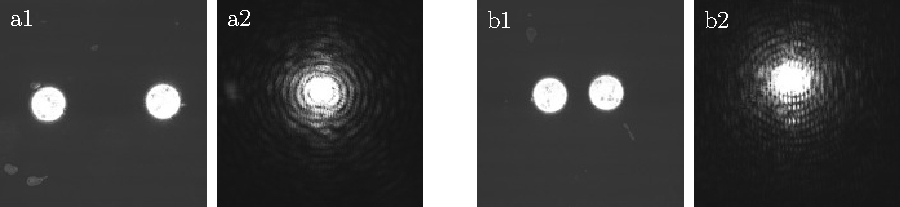
\includegraphics{images/Regina/abb15.pdf}
	\caption[Punktpaare unterschiedlicher Abstände und Fourierspektren]{
		Punktpaare mit unterschiedlichen Abständen zueinander (a1, b1) und die dazugehörigen Beugungsbilder in der Fourierebene (a2, b2).
	}
	\label{fig:punktpaare_verschieden_und_spektren}
\end{figure}


\begin{figure}[h]
	\centering
	%\includegraphicsRS[width=0.3\linewidth]{images/Regina/abb16.jpg}
	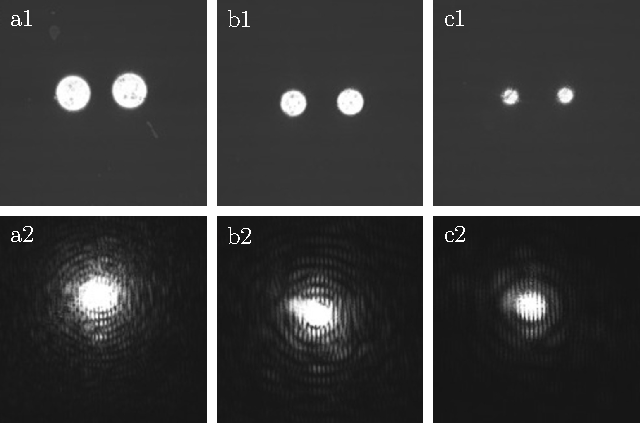
\includegraphics{images/Regina/abb16.pdf}
	\caption[Punktpaare gleicher Abstände und Fourierspektren]{
		Punktpaare mit gleichen Abständen und unterschiedlicher Größe (a1, b1, c1) und die dazugehörigen Beugungsbilder in der Fourierebene (a2, b2, c2).
	}
	\label{fig:punktpaare_gleich_und_spektren}
\end{figure}

Bei den geringsten Abstand sind im Beugungsbild neben den konzentrischen Formen auch vertikale Gitter zu erkennen (Abb.~\ref{fig:punktpaare_verschieden_und_spektren}~b2). Diese Gitterform stellen die bereits erwähnten Unterstrukturen der Beugungsbilder dar. Zwei Punkte ergeben in der Fourierebene als
Unterstruktur eine Linienstruktur senkrecht zur Verbindungslinie der beiden Punkte. Diese ergeben sich somit ebenfalls bei zwei Punkten mit höheren Abstand, sind aber wegen des kleinen Abstand zwischen den Spalten des vertikalen Gitters in der Fourierebene schlecht zu erkennen, da sich die Fouriertransformierte reziprok verhält (Ähnlichkeitstheorem). Bei kleinere Abstand zwischen den Punkten, vergrößert sich der Abstand der Spalten im vertikalen Gitter, und ist dadurch erkennbar. Diese Unterstrukturen sind noch ausgeprägter bei gleichbleibenden Abstand und kleinerer Größe der Punkte zu erkennen (Abb.~\ref{fig:punktpaare_gleich_und_spektren}~b2, c2). Die Intensitätsmaxima sind bei den kleineren Punkte durch ihren größeren Abstand zueinander kleiner ausgeprägt als bei den größeren Punkten. Somit weist das Hauptmotiv des Beugungsbild eine geringe Intensität auf, wodurch die Unterstruktur einfacher zu erkennen
ist.
Auch bei dem Beugungsbild eines Punktringes (Abb.~\ref{fig:punktringe_und_spektrum}) sind Unterstrukturen in der Fourierebene zu erkennen, die sich durch die Anordnung der acht Punkte ergeben. Zwei Punkte weisen eine senkrechte Linienstruktur zur Verbindungslinie auf, so dass sich bei acht Punkten vier Linienstrukturen (horizontal, vertikal, beide Diagonale) ergeben. Wenn sich diese Strukturen kreuzen, ergeben sich acht Schnittpunkte und somit eine Unterstrukturen, die wie Achtecke aussehen (Abb.~\ref{fig:punktringe_ausschnitt}).

\begin{figure}[h]
	\centering
	%\includegraphicsRS[width=0.10\linewidth]{images/Regina/abb17.jpg}
	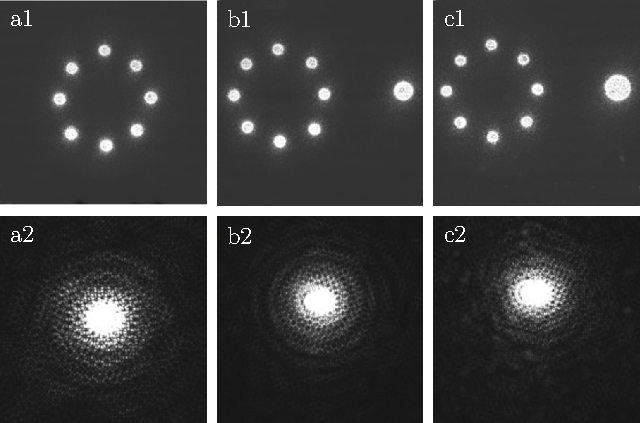
\includegraphics{images/Regina/abb17.pdf}
	\caption[Punktringe mit Fourierspektren]{
		Punktringe (a1) und Punktringe mit zusätzlichem Punkt in unterschiedlicher Größe (b1, c1) und die dazugehörigen Beugungsbilder in der Fourierebene (a2-c2).
	}
	\label{fig:punktringe_und_spektrum}
\end{figure}

\begin{figure}[h]
	\centering
	\includegraphicsRS[width=0.42\textwidth]{images/Regina/abb18.jpg}
	\caption[Beugungsbild der Punktringe mit vergrößertem Ausschnitt]{
		Ausschnitt aus dem Beugungsbild des Punktringes, welche die Unterstruktur eines Achtecks zeigt.
	}
	\label{fig:punktringe_ausschnitt}
\end{figure}

Bei einem Punktkreis mit einem zusätzlichen Punkt ist das Beugungsbild nicht mehr symmetrisch und die Asymmetrie nimmt mit größer werdenden Punkt zu (Abb.~\ref{fig:punktpaare_gleich_und_spektren}~b, c).


\subsection{Erzeugung von Beugungsbilder von Buchstaben und Zahlen}
\subsubsection*{Auswertung}

Der Buchstabe D besteht aus sowohl horizontalen, vertikalen Linien und runden Elementen (Abb.~\ref{fig:ziffern_mit_spektren}~a1). Das Beugungsbild ergibt sich somit aus der Summe der Beugungsbilder dieser verschiedenen Formen. Die horizontalen Linien bilden ein Fourierspektrum in der Horizontalen und die vertikalen Linien in der Vertikalen mit den jeweiligen Maxima und Minima und Unterstrukturen (Abb.~\ref{fig:ziffern_mit_spektren}~a2). Die runde Form erzeugt in dem Beugungsbild konzentrische Ringe mit abnehmender Intensität, entsprechend dem Beugungsbild von Punkten. Da der Buchstabe D durch horizontale und vertikalen Linien dominiert wird, ist auch das Beugungsbild stark davon geprägt, so dass die konzentrischen Ringe durch eine geringere Intensität auch schlechter zu erkennen sind.

\begin{figure}[h]
	\centering
	%\includegraphicsRS[width=0.4\textwidth]{images/Regina/abb19.jpg}
	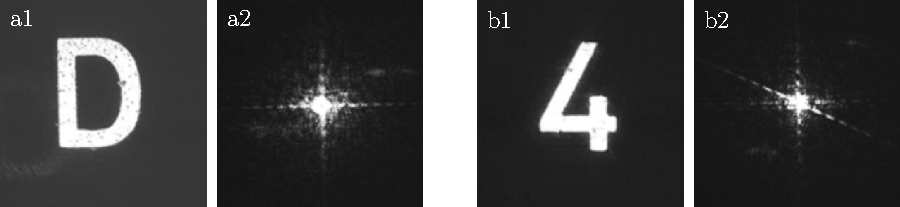
\includegraphics{images/Regina/abb19.pdf}
	\caption[Ziffern mit Fourierspektren]{
		Buchstabe D (a1) und Zahl 4 (b1) und die dazugehörigen Beugungsbilder in der Fourierebene (a2 und b2).
	}
	\label{fig:ziffern_mit_spektren}
\end{figure}

Die Zahl 4 besteht lediglich aus Linien, wobei neben horizontalen und vertikalen Linien ebenfalls diagonale Linien vorhanden sind (Abb.~\ref{fig:ziffern_mit_spektren}~b1). Da das erzeugten Beugungsbild eines Gitters eine senkrecht auf dem Gitter stehende Punktereiche aus Interferenzmaxima und –minima darstellt, ist zusätzlich zu der horizontalen und vertikalen Richtung ein Fourierspektrum in der Diagonalen senkrecht zur der Diagonale der Objektebene anzufinden (Abb.~\ref{fig:ziffern_mit_spektren}~b2).

\subsection{Erzeugung von Beugungsbildern des Fourierhauses}
\subsubsection*{Auswertung}

Das Fourierhaus ist ein Haus, welches aus Gittern mit gleichen Gitterkonstanten und unterschiedlicher Ausrichtungen der Gitter besteht (Abb.~\ref{fig:fourierhaus_mit_filtern}~a1). Die verschiedenen Gitter entsprechen verschiedenen Bauelementen im Haus. Die Wand besteht aus einem vertikalen Gitter, das Dach aus einem horizontalen Gitter und die Tür und der Schornstein werden aus diagonalen Gittern in entgegen gerichteten Richtung erstellt. Die Fouriertransformation dieses Fourierhauses ergibt das in Abbildung~\ref{fig:fourierhaus_mit_filtern}a2 dargestellte Beugungsbild. Die vier verschiedenen Orientierung der Gitter sind in der Fourierebene ebenfalls durch vier verschiedene Orientierungen dargestellt, die jeweils senkrecht auf der Objektebene stehen. Da die Gitterkonstante des Fourierhauses im Vergleich zu den in Abbildung~\ref{fig:gitter_und_spektrum} und \ref{fig:kreuzgitter_und_spektrum} gezeigten Gittern sehr viel kleiner ist, sind die Abstände zwischen den Maxima im Fourierspektrum deutlich größer (siehe 1.1. Ähnlichkeit%TODO REF!!!
 ) und die Intensität im Zentrum erhöht.


\subsection{Optische Filterung des Fourierhauses durch eine Schneide}
\subsubsection*{Auswertung}

Für eine optische Filterung wurden verschiedene Filter in der Fourierebene des 4f-Aufbaus eingesetzt (siehe Abb.4%TODO:REF!!!
). Zuerst wurde das Fourierhaus durch Filter manipuliert. Durch die Verwendung einer Schneide, die bestimmte Frequenzbereiche durch das Abdecken der Frequenzspektren durch lichtundurchlässigen Material herausfiltert, konnten verschieden Bauelemente jeweils heraus gefiltert werden. Durch zwei Schneiden wurden in dem Fourierebene das Beugungsbild so abgedeckt, dass lediglich das vertikale Fourierspektrum des Daches und das diagonale Fourierspektrum der Tür übrig blieben (Abb.~\ref{fig:fourierhaus_und_spektrum}~b1). Somit waren in der Abbildungsebene nur die näherungsweise horizontalen Linien des Daches und der Tür sichtbar (Abb.~\ref{fig:fourierhaus_und_spektrum}~b2). Analog wurden durch das Abdecken mit dem Filter erreicht, dass nur das horizontale Fourierspektrum sichtbar war und somit nur vertikale Linien (Wand) in der Abbildungsebene sichtbar wurden (Abb.~\ref{fig:fourierhaus_und_spektrum}~c1, c2). Als letztes wurde, durch das Blockieren des diagonalen Fourierspektrums, lediglich der Schonstein ausgeblendet (Abb.~\ref{fig:fourierhaus_und_spektrum}~d1, d2).

\begin{figure}[h]
	\centering
	%\includegraphicsRS[width=0.75\textwidth]{images/Regina/abb21.jpg}
	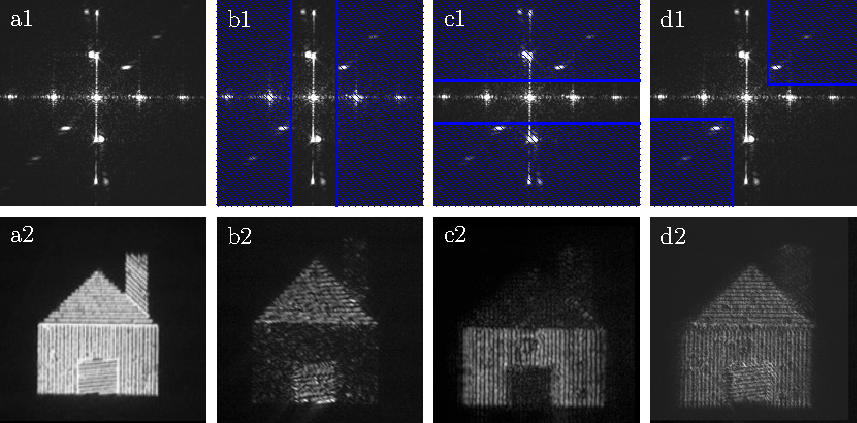
\includegraphics[scale=1]{images/Regina/abb21.pdf}
	
	\caption[Fourierhaus mit verschiedenen Filtern]{
		Durch zwei Schneiden (blau schraffiert) werden verschiedene Teile der Fourierspektren in der Fourierebene herausgefiltert (oben), welches in der Abbildungsebene zum Verschwinden einzelner Teile führt (unten).
	}
	\label{fig:fourierhaus_mit_filtern}
\end{figure}

\subsection{Optische Filterung durch Hochpass-, Tiefpass- und Breitbandfilter}

Als Nächstes wurde die Abbildung eines Fingerabdrucks auf einem Glasplättchen zunächst ohne Filter aufgenommen. Hierbei war in der Abbildungsebene relativ wenig zu erkennen (siehe Abbildung \ref{fig:example20_Hochpass}~a). Anschließend wurde die Abbildung mit einem in der Fourierebene befindlichen Hochpass- und einem Halbebenenfilter aufgenommen. Zudem wird mit Kamera 2 das Fourierspektrum des Fingerabdrucks photographiert. Zu beobachten war hier, dass die Konturen des Fingerabdrucks in der Abbildung mit Hilfe der Filter deutlich besser erkennbar gemacht werden konnten (vgl Abbildung \ref{fig:example20_Hochpass}~b, c).\\


\begin{figure}[h]
	\centering
	%\includegraphicsRS[width=0.6\linewidth]{images/example20_Hochpass.png}\\
	%\includegraphicsRS[width=0.6\linewidth]{images/example21_Halbebenenfilter.png}
	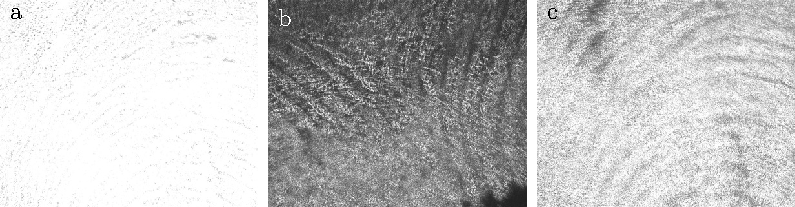
\includegraphics{images/ergebniss_Fingerab/abb.pdf}
	%TODO: Nur eines dieser Bilder!
	\caption{
		Der Fettabdruck eines Fingers in der Abbildungsebene ohne Filter (a) und mit Hochpassfiltern (b, c).
	}
	\label{fig:example20_Hochpass}
\end{figure}

\subsubsection*{Auswertung}

Als Erstes wird ein Breitbandfilter bei der Zahl vier eingesetzt. Da der Breitbandfilter sowohl kleinere und größere Frequenzen herausfiltert und somit nur eine bestimmtes Frequenzintervall durchlässt, werden die Flächen unterdrückt und Ränder als Doppellinien dargestellt. Beim Breitbandfilter C (Abb %TODO REF!!!
c) konnte dieser Effekt am besten beobachtet werden (Abb.~\ref{fig:vier_mit_breitband}~b). Bei den Breitbandfilter B und A ist die Filterwirkung so stark, dass nur
ein sehr kleiner Frequenzintervall durchgelassen wird und dadurch die Zahl vier kaum noch zu erkennen ist (Abb. \ref{fig:vier_mit_breitband}c, d).

\begin{figure}[h]
	\centering
	%\includegraphicsRS[width=0.4\textwidth]{images/Regina/abb22.jpg}
	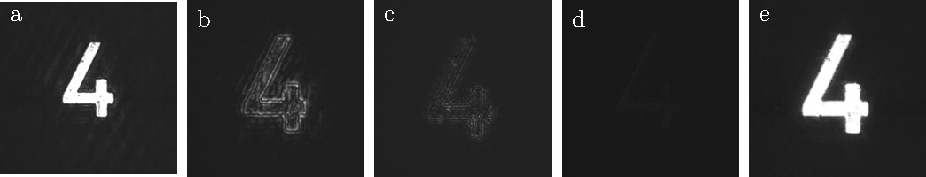
\includegraphics{images/Regina/abb22.pdf}
	\caption[Zahl 4 mit Breitbandfiltern]{
		Die Zahl vier in  der Abbildungsebene ohne Filter (a) und mit dem Breitbandfilter C (b), B (c) und A (d) gefilterte Bilder der Zahl vier.
	}
	\label{fig:vier_mit_breitband}
\end{figure}

Durch die Verwendung eines Tiefpassfilters wurden die niedrigen Frequenzen durchgelassen und somit die hohen Frequenzen herausgefiltert. Diese bewirken eine niedrigere Auflösung des
Bildes, da die Flächen unterdrückt werden, welches in der Abbildung~\ref{fig:vier_mit_breitband}~b dargestellt ist bei der Zahl 4 und dem Buchstaben D dargestellt ist. Da diese beiden Objekte keine innere Flächenstrukturen wie Gitter aufweisen, ist dieser Effekt nicht zu erkennen.
Im Gegenteil dazu wurden bei einem Fingerabdruck ein Hochpassfilter eingesetzt, der die niedrigen Frequenzen herausgefiltert, welches zu einer Hervorhebung der Kanten führte (Abb.~\ref{fig:vier_mit_tiefpass}~b). In der Bildverarbeitung werden die Tiefpass- (Weichzeichner) und Hochpassfilter (Kantenerkennung) häufig verwendet.

\begin{figure}[h]
	\centering
	%\includegraphicsRS[width=0.4\textwidth]{images/Regina/abb23.jpg}
	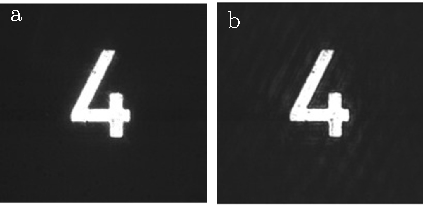
\includegraphics{images/Regina/abb23.pdf}
	\caption[Zahl 4 mit Tiefpassfilter]{
		Die Zahl vier in der Abbildungsebene (a) und mit dem Tiefpassfilter (b) gefilterte Abbildung der Zahl vier.
	}
	\label{fig:vier_mit_tiefpass}
\end{figure}


\begin{figure}[h]
	\centering
	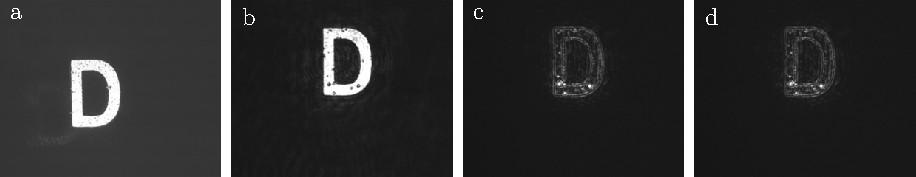
\includegraphics{images/ergebniss_D/abb.pdf}
	\caption{
		Der Buchstabe D des Objekts 4 in der Abbildungsebene ohne Filter (a), mit dem Filter 1D (b), 1C (c), 1B (d).
	}
	\label{fig:example10_Filter1B}
\end{figure}


\subsection{Schlierenverfahren durch Verwendung eines Halbebenenfilters}

Als Letztes wurde ein Teelicht auf die Position des Objektträgers gestellt und ein Halbebenenfilter in der Fourierebene installiert. Mit Kamera 1 wurden mehrere Abbildungen aufgenommen, um die Strömungsbewegungen oberhalb der Flamme beobachten zu können. Zum Vergleich wurde zudem eine Aufnahme mit Halbebenenfilter, jedoch ohne Teelicht gemacht (siehe Abb.~\ref{fig:Halbebenenfilter_mit_und_ohne_Teelicht}). Auf dieser Beispielaufnahme sind deutliche Verzerrungen des Lichts aufgrund der Luftströmungen über der Flamme des Teelichts zu erkennen. 

\begin{figure}[h]
	\centering
	%\includegraphicsRS[width=0.7\linewidth]{images/example22_Halbebenenfilter_mit_und_ohne_Teelicht.png}
	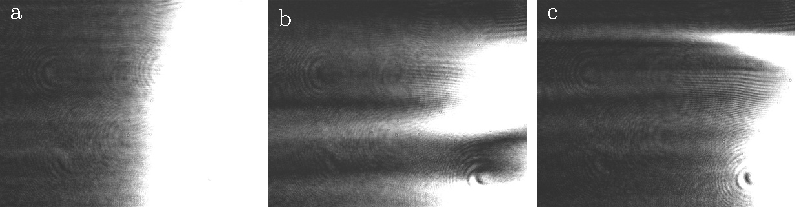
\includegraphics{images/ergebniss_Teelicht/abb.pdf}
	\caption[Schlieren]{
		Aufnahme ohne Objekt in der Abbildungsebene mit Halbebenenfilter ohne Teelicht (a) und mit Teelicht (b, c).
	}
	\label{fig:Halbebenenfilter_mit_und_ohne_Teelicht}
\end{figure}


\subsubsection*{Auswertung}

Mit Hilfe eines Halbebenenfilters (Schneide) wurden die durch   eine brennende Kerze erzeugten Schlieren dargestellt (Abb.~\ref{fig:Halbebenenfilter_mit_und_ohne_Teelicht}). Als Schlieren werden Bereiche bezeichnet, die sich von ihrer Umgebung  in  der  Dichte  bzw.  im  Brechungsindex  unterscheiden,  welche  in  unseren Versuch die durch  die  Kerze erzeugten Luftströmungen darstellten. Bei diesem Versuchsaufbau  wurde  das  Prinzip  genutzt,  dass  parallele  Strahlenbündel  beim  Durchgang durch   ein   inhomogenes Dichtefeld   unterschiedlich   stark   abgelenkt   werden.   Durch   die eingesetzte  Schneide,  wurden  die  Anteile  des  gebrochenen  Lichts  ausgeblendet,  so  dass richtungsabhängige  Brechzahl-  bzw.  Dichtegradienten auf  dem  Projektionsschirm  sichtbar wurden. Dabei ist die Intensitätsverteilung im   Bild   proportional   zum   Quadrat   der Phasenverschiebung   durch   das   Objekt.   Somit   ermöglicht es dieses Verfahren, eine Phasenverschiebung sichtbar zu machen. 
